\documentclass[12pt]{article} % 12 -- размер шрифта
\usepackage{cmap} % Чтобы можно было копировать русский текст из pdf
\usepackage[T2A]{fontenc}
\usepackage[russian]{babel} % В частности эта строка отвечает за правильные переносы слов в конце строки
\usepackage[utf8]{inputenc} % Проверьте, что кодировка файла -- тоже utf8
\usepackage{amsmath, amssymb} % Чтобы юзать математические символы
\usepackage{ dsfont }
\usepackage{ wasysym }
\usepackage[makeroom]{cancel}
\usepackage{listings}
\usepackage{tcolorbox}

\usepackage[utf8]{inputenc}

\usepackage{listings}
\usepackage{xcolor}
\usepackage{tikz}
\usetikzlibrary {positioning}

\newcommand \tab[1][1cm]{\hspace*{#1}}

\definecolor{codegreen}{rgb}{0,0.6,0}
\definecolor{codegray}{rgb}{0.94, 0.94, 0.92}
\definecolor{codepurple}{rgb}{0.92,0,0.54}
\definecolor{backcolour}{rgb}{0.95,0.95,0.92}

\lstdefinestyle{mystyle}{
	backgroundcolor=\color{backcolour},   
	commentstyle=\color{codegreen},
	keywordstyle=\color{magenta},
	numberstyle=\tiny\color{codegray},
	stringstyle=\color{codepurple},
	basicstyle=\ttfamily\footnotesize,
	breakatwhitespace=false,         
	breaklines=true,                 
	captionpos=b,                    
	keepspaces=true,                 
	numbers=left,                    
	numbersep=5pt,                  
	showspaces=false,                
	showstringspaces=false,
	showtabs=false,                  
	tabsize=2
}

\lstset{style=mystyle}

\graphicspath{ {./images/} }

\begin{document}

\title{Рекурсия}
\author{Парамонов Антон Игоревич}
\maketitle

\section{Введение}

Один из самых ярких примеров рекурсии в жизни - это матрешка.\\

\begin{tikzpicture}
\begin{scope}
	\clip [rounded corners=.5cm] (0,0) rectangle coordinate (centerpoint) (9, 9cm); 
	\node [inner sep=0pt] at (centerpoint) {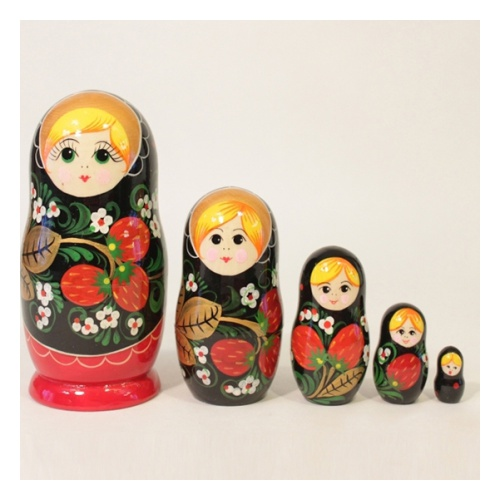
\includegraphics[width=10.0cm]{matreshka.jpg}}; 
\end{scope}
\end{tikzpicture}\\

Рекурсия - это отражение принципа самоподобия в программировании, давайте разберемся, где же у программы появляется возможность повторить саму себя.

Для этого вспомним функции. Мы говорили, что в теле функции можно писать любую программу, но ведь тогда в теле функции можно вызвать эту же функцию! Такой вызов функции самой себя называется \textit{рекурсивным} вызовом. Рассмотрим пример
\begin{lstlisting}[language=Python]
def f():
	print(42)
	f()
	

f()
\end{lstlisting}
Как работает такая программа? Сначала вызывается функция \colorbox{codegray}{f}, она печатает 42, после чего вызывается функция \colorbox{codegray}{f}, она печатает 42, после чего вызывается функция \colorbox{codegray}{f}... понятно, что так будет продолжаться бесконечно долго. Давайте изобразим происходящее с помощью таблицы\\
\\
\begin{tabular}{|l|l|}
	\hline
	Номер вызова & Печать \\
	\hline
	1 & 42 \\
	\hline
	2 & 42 \\
	\hline
	3 & 42 \\
	\hline
	\vdots & \vdots \\
	\hline
	$\infty$ & 42 \\
	\hline
\end{tabular}\\
\\
От такой программы, конечно, мало толку. Но давайте научимся останавливать рекурсию в нужный нам момент. Для этого у функции \colorbox{codegray}{f} заведем аргумент \colorbox{codegray}{n} - количество раз, которое мы еще хотим напечатать 42 до завершения.
\begin{lstlisting}[language=Python]
def f(n):
	if n == 0:
		return
	print(42)
	f(n - 1)


f(10)
\end{lstlisting}
Произошло два изменения: во-первых, если вызывается \colorbox{codegray}{f(0)}, то по нашему желанию функция должна печатать 42 еще 0 раз, т.е. не печатать вовсе, т.е. просто сделать \colorbox{codegray}{\textcolor{codepurple}{return}}. Этой логикой и занимается \colorbox{codegray}{\textcolor{codepurple}{if}} во второй строчке.\\
Во-вторых, когда функция, которой нужно было напечатать 42 n раз, произвела \colorbox{codegray}{\textcolor{codepurple}{print}(42)}, ее потомкам осталось сделать n - 1 \colorbox{codegray}{\textcolor{codepurple}{print}(42)}, так что в строчке 5 мы вызываем \colorbox{codegray}{f(n - 1)}. Вот как теперь выглядит табличка\\
\\
\begin{tabular}{|l|l|l|}
	\hline
	Номер вызова & Печать & n \\
	\hline
	1 & 42 & 10\\
	\hline
	2 & 42 & 9\\
	\hline
	3 & 42 & 8\\
	\hline
	\vdots & \vdots & \vdots \\
	\hline
	10 & 42 & 1 \\
	\hline
	11 & - & 0\\
	\hline
\end{tabular}\\
\\
Заметьте, что конечности мы добились благодаря тому, что в действительности функция, хоть и вызывает саму себя, но каждый раз с новым аргументом и зацикливания/повторения состояния не происходит.\\
\\
\textit{\textcolor{purple}{Вопрос на подумать}}: а что бы произошло, вызови мы функцию не от 10, как в примере, а от -1?\\
\begin{tcolorbox}[colback=white, colframe=black]
	\textit{Шутка}\\
	Чтобы понять рекурсию, нужно понять рекурсию.
\end{tcolorbox}

\section{Применение}
Теперь научимся решать с помощью рекурсии полезные задачи.\\
\begin{tcolorbox}[colback=white, colframe=black]
	\textit{Задача}\\
	Вводится число $n$, требуется посчитать сумму $1 + 2 + 3 + \ldots + n$.
\end{tcolorbox}
Конечно, многие из вас знают формулу
\begin{align*}
1 + 2 + 3 + \ldots + n = \frac{n\cdot(n + 1)}{2}
\end{align*}
а те, кто не знают, могут предложить решить эту задачу с помощью цикла. Но мы сейчас решим использовав рекурсию!\\
Для этого заведем название для этой суммы: 
\begin{align*}
\mathrm{sum}(n) := 1 + 2 + 3 + \ldots + n - 1 + n
\end{align*}
И расставим скобки: 
\begin{align*}
1 + 2 + 3 + \ldots + n - 1 + n = (1 + 2 + 3 + \ldots + n - 1) + n
\end{align*}
Ну и что, спросите вы? Это же очевидно. А то, что в скобках стоит ни что иное как $\mathrm{sum}(n - 1)$! И мы получаем \textit{рекурентную} формулу:
\begin{align}
\mathrm{sum}(n) = \mathrm{sum}(n - 1) + n
\end{align}

Чем-то напоминает динамику, правда? Давайте попробуем это написать
\begin{lstlisting}[language=Python]
def sum(n):
	return sum(n - 1) + n
\end{lstlisting}
Лаконично и изящно. Однако, к сожалению, неверно. Чтобы понять, где мы допустили ошибку, попробуем промоделировать работу программы при запуске \colorbox{codegray}{f(3)}. Пользуясь формулой (1), получим\\
$
\mathrm{sum}(3) =\newline \mathrm{sum}(2) + 3 = \text{\textcolor{gray}{/раскроем sum(2)/}} \newline \mathrm{sum}(1) + 2 + 3 =\text{\textcolor{gray}{/раскроем sum(1)/}}\newline \mathrm{sum}(0) + 1 + 2 + 3 = \newline \mathrm{sum}(-1) + 0 + 1 + 2 + 3 =\newline \mathrm{sum}(-2) + (-1) + 0 + 1 + 2 + 3 = \newline \ldots
$\\
Мы просто никогда не останавливаемся! Исправить это очень просто, нужно лишь заметить, что сумма чисел от 1 до 1 равна 1, или $\mathrm{sum}(1) = 1$. Учтем это в коде
\begin{lstlisting}[language=Python]
def sum(n):
	if n == 1:
		return 1
	return sum(n - 1) + n
\end{lstlisting}
Подобная тонкость еще раз напоминает нам динамику, в которой необходимо было указывать начальное условие. Но если динамика начинала с такого условия, то рекурсия им заканчивает, так что в случае с рекурсией этот \colorbox{codegray}{\textcolor{codepurple}{if}} называется заканчивающим или \textit{терминирующим} условием.\\
Вообще, рекурсия и динамика очень похожи, только динамика считает от 1 до n, а рекурсия - от n до 1. 
\section{Ошибка в Python}
Если вы забыли завести останавливающий \colorbox{codegray}{\textcolor{codepurple}{if}}, и ваша функция вызывается раз за разом, создавая бесконечную рекурсию, умный Python не даст вашему компьютеру сломаться, а остановит программу с ошибкой\\
\colorbox{codegray}{\textcolor{red}{RecursionError: maximum recursion depth exceeded}}\\
В вашем арсенале появился новый способ сломать программу!:)
\end{document}